\documentclass[tikz, border=2mm]{standalone}

\usepackage{mathpazo}
\usepackage{helvet}
\usetikzlibrary{decorations.pathmorphing}
\usetikzlibrary{decorations.pathreplacing}
\usetikzlibrary{shapes.symbols}

\begin{document}%

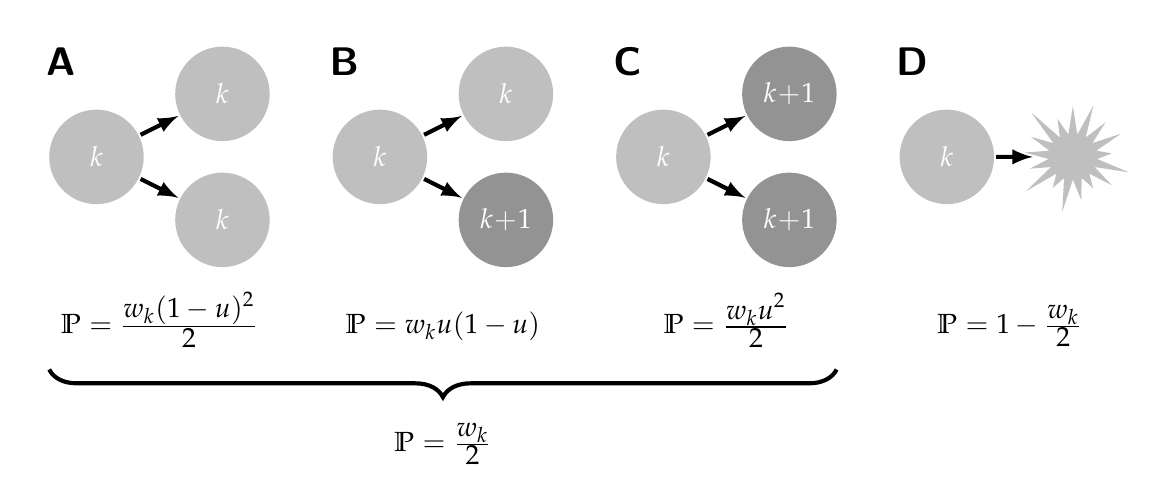
\begin{tikzpicture}[line width=1.5pt]

% Help lines
% \draw[help lines, dashed] (-1, -4) grid (13, 2);

% Labels
\node[right] (A)          at      (-0.9, 1.21) [circle]  {\Large\sf\textbf{A}};
\node[right] (B)          at       (2.7, 1.21) [circle]  {\Large\sf\textbf{B}};
\node[right] (C)          at       (6.3, 1.21) [circle]  {\Large\sf\textbf{C}};
\node[right] (D)          at       (9.9, 1.21) [circle]  {\Large\sf\textbf{D}};

% A
\node (par1)       at       (0, 0)      [circle, minimum size=12mm, fill=gray!50]      {\textcolor{white}{$k$}};
\node (off11)      at       (1.6, .8)   [circle, minimum size=12mm, fill=gray!50]      {\textcolor{white}{$k$}};
\node (off12)      at       (1.6, -.8)  [circle, minimum size=12mm, fill=gray!50]      {\textcolor{white}{$k$}};
\draw[-latex]  (par1)  to  (off11);
\draw[-latex]  (par1)  to  (off12);

% B
\node (par2)       at       (3.6, 0)    [circle, minimum size=12mm, fill=gray!50]      {\textcolor{white}{$k$}};
\node (off21)      at       (5.2, .8)   [circle, minimum size=12mm, fill=gray!50]      {\textcolor{white}{$k$}};
\node (off22)      at       (5.2, -.8)  [circle, minimum size=12mm,fill=gray!85]      {\textcolor{white}{$k\!+\!1$}};
\draw[-latex]  (par2)  to  (off21);
\draw[-latex]  (par2)  to  (off22);

% C
\node (par3)       at       (7.2, 0)    [circle, minimum size=12mm, fill=gray!50]      {\textcolor{white}{$k$}};
\node (off31)      at       (8.8, .8)     [circle, minimum size=12mm, fill=gray!85]      {\textcolor{white}{$k\!+\!1$}};
\node (off32)      at       (8.8, -.8)    [circle, minimum size=12mm, fill=gray!85]      {\textcolor{white}{$k\!+\!1$}};
\draw[-latex]  (par3)  to  (off31);
\draw[-latex]  (par3)  to  (off32);

% D
\node (ind)        at       (10.8, 0)    [circle, minimum size=12mm, fill=gray!50]      {\textcolor{white}{$k$}};
\node (dead)       at       (12.4, 0)   [starburst, minimum size=3mm, fill=gray!50]      {\textcolor{gray!50}{$n$}};
\draw[-latex]  (ind)  to  (dead);

% Probabilities
\node (p1)  at       (0.8, -2.07)      {$\mathbb{P} = \frac{\displaystyle w_k (1-u)^2}{\displaystyle 2}$};
\node (p2)  at       (4.4, -2.15)      {$\mathbb{P} = w_k u (1-u)$};
\node (p3)  at       (8.0, -2.08)      {$\mathbb{P} = \frac{\displaystyle w_k u^2}{\displaystyle 2}$};
\node (p4)  at      (11.6, -2.15)      {$\mathbb{P} = 1-\frac{\displaystyle w_k}{\displaystyle 2}$};

\draw [decorate,decoration={brace,amplitude=10pt}]
 (9.4,-2.7) -- (-0.6,-2.7) node [black,midway,yshift=-27pt] 
{$\mathbb{P} = \frac{\displaystyle w_k}{\displaystyle 2}$};

\end{tikzpicture}

\end{document}